\documentclass[__main__.tex]{subfiles}

\begin{document}

\qtitle{С}{01}
Электрический диполь: электрический дипольный момент, потенциальная энергия диполя в электростатическом поле, момент сил, действующих на диполь в однородном электростатическом поле.\\

\textbf{Электрический диполь} — идеализированная электронейтральная система, состоящая из точечных и равных по абсолютной величине положительного и отрицательного электрических зарядов.

Другими словами, электрический диполь представляет собой совокупность двух равных по абсолютной величине разноимённых точечных зарядов, находящихся на некотором расстоянии друг от друга

Произведение вектора $ \vec l$, проведённого от отрицательного заряда к положительному, на абсолютную величину зарядов $ q\,,$ называется \textbf{дипольным моментом}: $\vec d=q\vec l$.

Во внешнем электрическом поле $\vec E$ на электрический диполь действует момент сил ${\vec d}\times{\vec E}$, который стремится повернуть его так, чтобы дипольный момент развернулся вдоль направления поля.

Потенциальная энергия электрического диполя в (постоянном) электрическом поле равна $-{\vec E}\cdot{\vec d}$. (В случае неоднородного поля это означает зависимость не только от момента диполя - его величины и направления, но и от места, точки нахождения диполя).

Вдали от электрического диполя напряжённость его электрического поля убывает с расстоянием $R$ как $R^{-3}$, то есть быстрее, чем у точечного заряда ( $E \sim R^{-2}$).

Любая в целом электронейтральная система, содержащая электрические заряды, в некотором приближении (то есть собственно в дипольном приближении) может рассматриваться как электрический диполь с моментом $\vec d = \sum_i q_i {\vec r}_i$, где $q_{i}$ — заряд $i$-го элемента, ${\vec r}_i$ — его радиус-вектор. При этом дипольное приближение будет корректным, если расстояние, на котором изучается электрическое поле системы, велико по сравнению с её характерными размерами.
\\
Найдём \textbf{потенциальную энергию}, которой обладает диполь во внешнем электрическом поле (см. Рисунок 1). Эта энергия будет равна:

\begin{equation}
    \textit{П} = q\varphi_+ - q\varphi_- = q(\varphi_+ - \varphi_-),
    \llabel{eq:1}
\end{equation}

где $\varphi_+$ и $\varphi_-$ - значения потенциалов внегнего поля в точках, где находятся заряды $+q$ и $-q$.

\begin{equation}
    \varphi_+ - \varphi_- = \frac{d\varphi}{dx} \Delta x = \frac{d\varphi}{dx} l \cos \alpha.
    \llabel{eq:2}
\end{equation}

\begin{figure}[h]
    \centering
    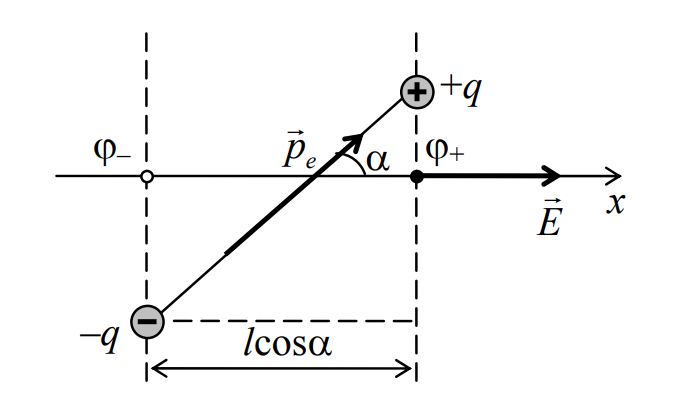
\includegraphics[width=.6\linewidth]{e01_1.png}
    \caption{ }
    \llabel{fig:1}
\end{figure}

Подставив выражение (\lref{eq:2}) в (\lref{eq:1}) и учитывая, что $E = -\frac{d\varphi}{dx}$, получим:

\begin{equation}
    \textit{П} = q\frac{d\varphi}{dx} l \cos \alpha = -qEl\cos \alpha = -p_e E \cos \alpha
    \llabel{eq:3}
\end{equation}

Так как угол $\alpha$ в формуле (\lref{eq:3}) - это угол между векторами $\vec{E}$ и $\vec{p_e}$, то данное выражение можно записать в виде:

\begin{equation}
    \textit{П} = - \vec{p_e} \vec{E}
    \llabel{eq:4}
\end{equation}

Выражение (\lref{eq:4}) не учитывает энергию взаимодействия зарядов $+q$ и $-q$, образующих диполь.

Рассмотрим поведение диполя во внешнем электрическом поле. Если диполь поместить в однородное электрическое поле, образующие диполь заряды $+q$ и $-q$ окажутся под дейстивем равных по величине, но противоположных по направлению сил $\vec{F_1}$ и $\vec{F_2}$ (см. Рис. \lref{fig:2}).
\textbf{Момент пары сил}, действующих на диполь, будет равен:

\begin{equation}
    M = Fd = Fl\sin \alpha = qEl\sin \alpha = p_e E \sin \alpha,
    \llabel{eq:5}
\end{equation}
где $d = l\sin \alpha$ - момент пары сил.

\begin{figure}[h]
    \centering
    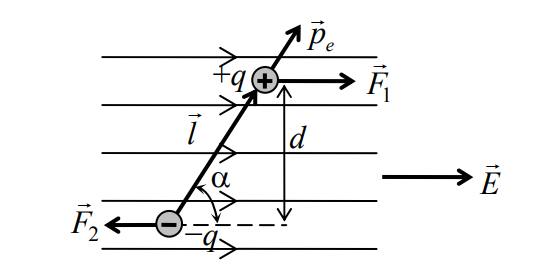
\includegraphics[width=.6\linewidth]{e01_2.png}
    \caption{ }
    \llabel{fig:2}
\end{figure}

Формулу (\lref{eq:5}) можно записать в векторном виде:

\begin{equation}
    \vec{M} = \vec{p_e} \times \vec{E}.
\end{equation}

Момент сил стремится повернуть диполь так, чтобы его электрический момент $\vec{p_e}$ установился по направлению поля.

\end{document}